s\documentclass{article}
\usepackage{graphicx}
\usepackage{amsmath}
\usepackage{listings}
\usepackage{geometry}
\usepackage{physics}
\usepackage[utf8]{inputenc}

\geometry{
 a4paper,
 total={170mm,257mm},
 left=20mm,
 top=20mm,
 }

\title{Assignment 6: The Laplace Transform }
\author{Jineeth N [EE20B051]}
\date{\today}

\begin{document}

\maketitle % Insert the title, author and date		

\section{Introduction}
 In this assignment, we will analyze Linear Time-Invariant systems using scipy library in python. Our analysis will be mostly based on polynomial transfer functions

\section{Tasks}
\subsection{Forced oscillatory system}

\subsubsection{Impulse response}
    The system is characterized by given differential equation
    \begin{equation}
    \dv[2]{x}{t} + 2.25x = f(t) 
        \end{equation}
        
$f(t)$ is defined as,
    \begin{equation}
    f(t) = cos{(\omega t)}*\exp(-at)u(t)
        \end{equation}

    The laplace transform of input signal is,
    \begin{equation}
    F(s) = \frac{s+a}{(s+a)^2+2.25 }
        \end{equation}
        
    In the above equation '$a$' represents decay value. We will consider two different values 0.5, 0.05 for a and analyze the impulse response

\begin{verbatim}
    # The python code snippet for Q.1
    X1 = sp.lti([1, 0.5], polymul([1, 1, 2.5], [1, 0, 2.25]))
    t1, x1 = sp.impulse(X1, None, linspace(0, 50, 500))
    
    # The plot x(t) vs t for Q.1
    plt.figure(0)
    plt.plot(t1, x1)
    plt.title("Decay = 0.5")
    plt.xlabel("t")
    plt.ylabel("x(t)")
    plt.grid()
    
    # The python code snippet for Q.2
    X2 = sp.lti([1, 0.05], polymul([1, 0.1, 2.2525], [1, 0, 2.25]))
    t2, x2 = sp.impulse(X2, None, linspace(0, 50, 500))
    
    # The plot of x(t) vs t for Q.2
    plt.figure(1)
    plt.plot(t2, x2)
    plt.title("Decay = 0.05")
    plt.xlabel("t")
    plt.ylabel("x(t)")
    plt.grid(True)
\end{verbatim}


 \begin{figure}[!ht]
  \centering
  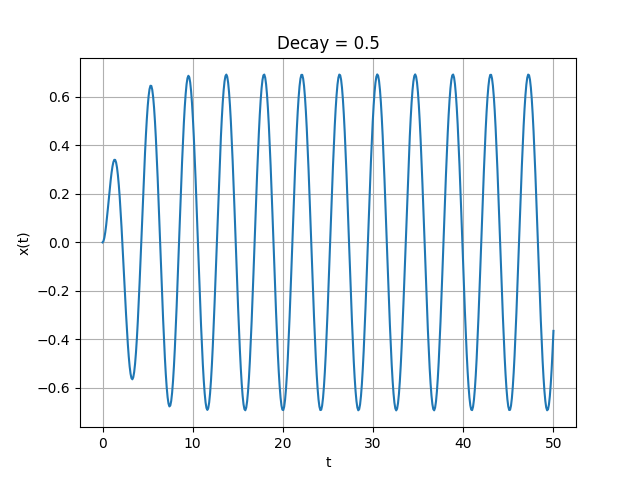
\includegraphics[scale=0.5]{Figure_0.png}
  \caption{Output for different frequencies}
  \label{fig:sample}
  \end{figure}
 \begin{figure}[!ht]
  \centering
  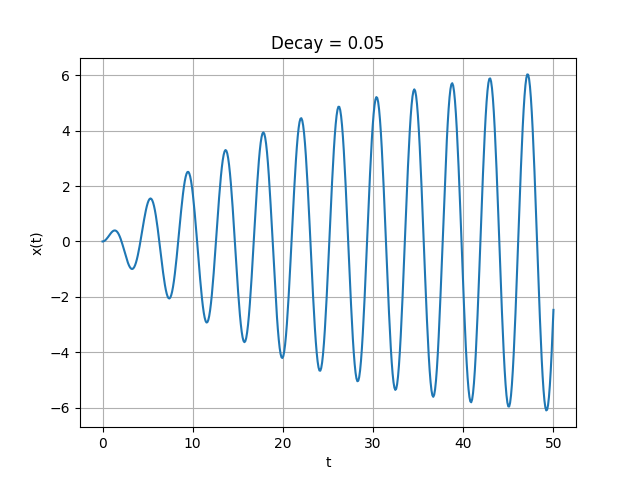
\includegraphics[scale=0.5]{Figure_1.png}
  \caption{Output for different frequencies}
  \label{fig:sample}
  \end{figure}
 
\newpage
\subsubsection{Responses for various frequencies}

    Now we will vary the frequency of the input signal from 1.4 to 1.6 and analyze the output response of the system using scipy.lsim function
\begin{verbatim}
    H = sp.lti([1], [1, 0, 2.25])
    l = 1.4
    r = 1.6
    for w in arange(l, r, 0.05):
    t = linspace(0, 80, 500)
    f = np.cos(w * t) * np.exp(-0.05 * t)
    t, x, svec = sp.lsim(H, f, t)

    # The plt.plot of x(t) for various frequencies vs time.
    plt.figure(2)
    plt.plot(t, x, label="w = " + str(w))
    plt.title("x(t) for various frequencies")
    plt.xlabel("t")
    plt.ylabel("x(t)")
    plt.legend()
    plt.grid(True)

\end{verbatim}
\begin{figure}[!ht]
  \centering
  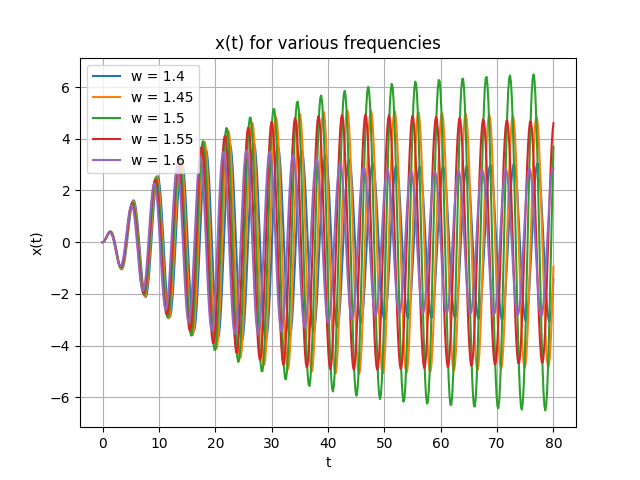
\includegraphics[scale=1]{Figure_2.png}
  \caption{Output for different frequencies}
  \label{fig:sample}
  \end{figure}
 
 \subsection{Coupled spring problem}
 In this problem we have two differential equations and two variables to solve for.
The equations are
\begin{equation}
\dv[2]{x}{t} +(x-y) = 0
\end{equation}
\begin{equation}
\dv[2]{y}{t} +2(y-x) = 0   
\end{equation}

With initial condition as x(0) = 1
On solving both equations we get,
\begin{equation}
   X(s) = \frac{s^2+2}{s^3+3s} 
\end{equation}
\begin{equation}
  Y(s) =  \frac{2}{s^3+3s}  
\end{equation}
 \begin{verbatim}
    t4 = linspace(0, 20, 500)
    X4, Y4 = sp.lti([1, 0, 2], [1, 0, 3, 0]), sp.lti([2], [1, 0, 3, 0])
    t4, x4 = sp.impulse(X4, None, t4)
    t4, y4 = sp.impulse(Y4, None, t4)
    
    # The plot of x(t) and y(t) vs t for Q.4
    plt.figure(3)
    plt.plot(t4, x4, label="x(t)")
    plt.plot(t4, y4, label="y(t)")
    plt.title("x(t) and y(t)")
    plt.xlabel("t")
    plt.ylabel("functions")
    plt.legend()
    plt.grid(True)
 \end{verbatim}
 
 \begin{figure}[!ht]
  \centering
  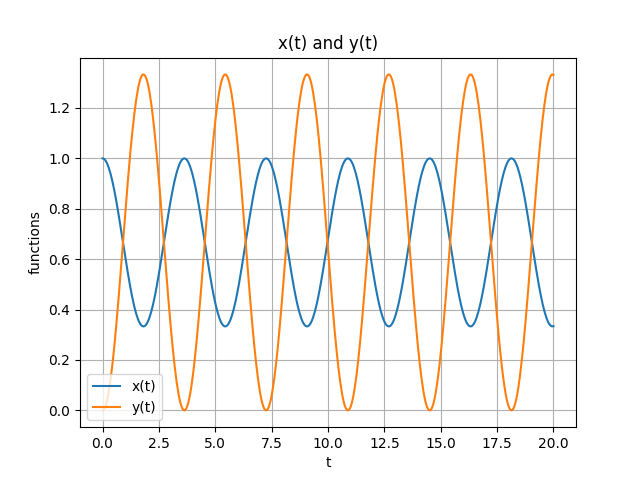
\includegraphics[scale=1]{Figure_3.png}
  \caption{Solutions of coupled spring equations}
  \label{fig:sample}
  \end{figure}

\subsection{Two port RLC Circuit}
\subsubsection{Bode plot of Steady State Transfer function}
We now consider the case of an RLC Filter with the transfer function as shown.
\begin{equation}
    H(s) = \frac{1}{10^{-12}s^2 + 10^{-4}s + 1}
\end{equation}
 
\subsubsection{Output voltage for given input signal}
The input is of the form
\begin{equation}
   x(t) = \cos{(10^3t)}-\cos{(10^6t)} 
\end{equation}
\begin{verbatim}
# The python code snippet for Q.6
t6 = arange(0, 25e-3, 1e-7)
vi = cos(1e3 * t6) - cos(1e6 * t6)
t6, vo, svec = sp.lsim(H5, vi, t6)

# The plot of Vo(t) vs t for large time interval.
plt.figure(6)
plt.plot(t6, vo)
plt.title("The Output Voltage for large time interval")
plt.xlabel("t")
plt.ylabel("V_o(t)")
plt.grid(True)

# The plot of Vo(t) vs t for small time interval.
plt.figure(7)
plt.plot(t6[0:350], vo[0:350])
plt.title("The Output Voltage for small time interval")
plt.xlabel("t")
plt.ylabel("V_o(t)")
plt.grid(True)
\end{verbatim}

\begin{figure}[!ht]
  \centering
  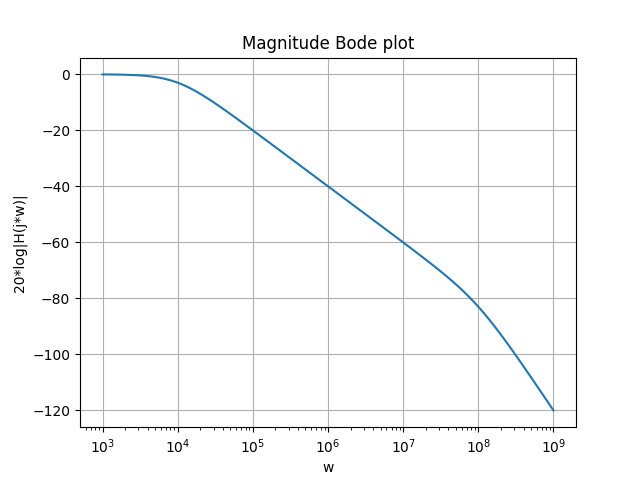
\includegraphics[scale=0.7]{Figure_4.png}
  \caption{Bode tranfer of transfer function in RLC circuit}
  \label{fig:sample}
  \end{figure}
  
 \begin{figure}[!ht]
  \centering
  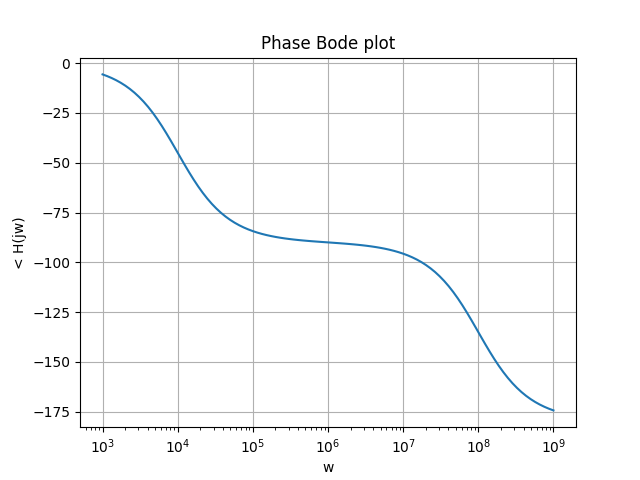
\includegraphics[scale=0.7]{Figure_5.png}
  \caption{Bode tranfer of transfer function in RLC circuit}
  \label{fig:sample}
  \end{figure}
 
 \section{Conclusion}
 The ripple in the signal in small time interval plot is because of the high frequency component. But the ripples are not visible in large time interval because the presence of low frequency component of which amplitude remained almost unchanged and dominated high frequency signal.


\begin{figure}[!ht]
  \centering
  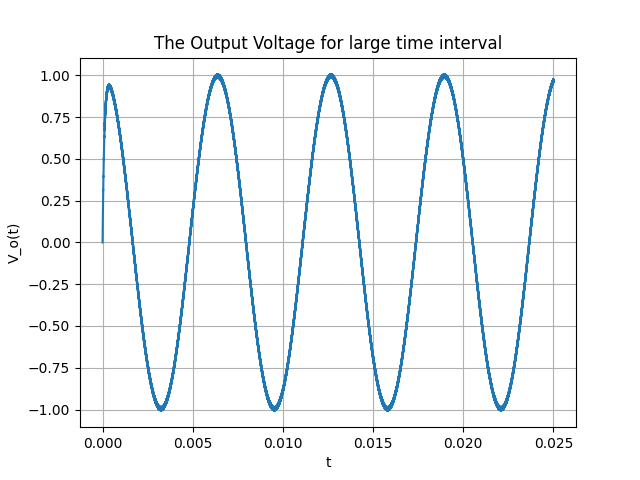
\includegraphics[scale=0.7]{Figure_6.png}
  \caption{Output voltage for t$<$20msec}
  \label{fig:sample}
  \end{figure}
  
 \begin{figure}[!ht]
  \centering
  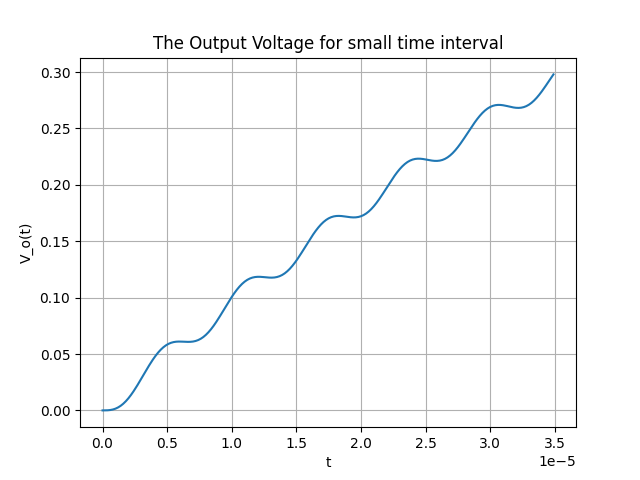
\includegraphics[scale=0.7]{Figure_7.png}
  \caption{Output voltage for t$<$10µsec}
  \label{fig:sample}
  \end{figure}
  
  
\end{document}